\documentclass[xcolor=pdftex,dvipsnames,table]{beamer}

\mode<presentation>
{
  \usetheme{Madrid}
  \usecolortheme{seagull}
  \setbeamercovered{dynamic} %invisible,transparent,dynamic,highly dynamic
}

%%%%%%%%%%%%%%%%%%%%%%%%%%%%%%%%%%%%%%%%
%%%%%%%%%%%% PACKAGES %%%%%%%%%%%%%%%%%%

\usepackage[utf8]{inputenc}

\usepackage[english]{babel}

\usepackage{amsmath,amsfonts,amssymb,amscd,amsthm, bm, stmaryrd}

\usepackage{listings}
\usepackage[cache=false,section]{minted}


\usepackage{multirow}

\usepackage{caption}
\usepackage{subcaption}

\usepackage{tikz}
\usetikzlibrary{external, automata, arrows.meta, positioning, calc}
\tikzexternalize[shell escape=-shell-escape,mode=graphics if exists, prefix=../thesis/tikz/cache/]
\newcommand{\inputtikz}[1]{%
  \tikzsetnextfilename{#1}%
  \input{../thesis/tikz/#1.tex}
}

\usepackage{graphicx}
\graphicspath{{../thesis/figures/}}

\usepackage{xcolor,colortbl}
\definecolor{Red}{rgb}{0.89, 0.0, 0.13}
\definecolor{Pink}{rgb}{1.0, 0.65, 0.79}
\definecolor{lightgreen}{rgb}{0.56, 0.93, 0.56}
\newcolumntype{a}{>{\columncolor{lightgreen}}c}
\newcolumntype{b}{>{\columncolor{Red}}c}

\newcommand{\code}[1]{\texttt{#1}}

%%%%%%%%%%%%%%%%%%%%%%%%%%%%%%%%%%%%%%
%%%%%%%%%%%%% TITLE %%%%%%%%%%%%%%%%%

\title{Distributed Complex Event Recognition}
\subtitle{Master's Thesis}
\author{Arnau Abella}
\institute[UPC]{%
  {\tiny %
    \textit{Supervisors:}\\
    Sergi Nadal, Universitat Politècnica de Catalunya\\
    Stijn Vansummeren, UHasselt – Hasselt University\\
  }
  \vspace{10pt}
  \textrm{\scriptsize%
    Master in innovation and research in informatics\\
    \vspace{5pt}
    Facultat d’Informàtica de Barcelona (FIB)\\
    Universitat Politècnica de Catalunya (UPC)\\
  }
}
\date{\tiny \today}

%%%%%%%%%%%%%%%%%%%%%%%%%%%%%%%%%%%%%%%%
%%%%%%%%%%%% DOCUMENT %%%%%%%%%%%%%%%%%%

\AtBeginSection[]
{
  \begin{frame}<beamer>
      \frametitle{Table of Contents}
      \tableofcontents[currentsection]
  \end{frame}
}

\begin{document}

\frame{\titlepage}

%%%%%%%%%%%%%%%%%%%%%%%%%%%%%%%%%%%%%%%%%%%%%%%%%%%%%%%%%%%%%%%%%%
%%%%%%%%%%%%%%%%%%%%%%%%%%%%%%%%%%%%%%%%%%%%%%%%%%%%%%%%%%%%%%%%%%

\section{Introduction}

\begin{frame}[fragile]{Introduction}
  \begin{block}{\emph{Complex Event Recognition (CER)}}
    Identifying collections of events that collectively satisfy some pattern in high-velocity streams.
  \end{block}

  \begin{block}{Features}
    Allow expressing patterns based on:
   \begin{itemize}
     \item Content
     \item Position in the stream
     \item Order w.r.t other events
     % \item More constraints
   \end{itemize}
  \end{block}
\end{frame}

\begin{frame}[fragile]{Introduction}
  \begin{example}
    A stream produced by wireless sensors placed in a warehouse, whose main objective is to detect fires.
    \begin{figure}[H]
      \centering
      \begin{tabular}{|c|c|c|c|c|c|c|c|c|c|c}\hline
        type  &$H$&$T$&$H$&$H$&$T$&$H$&$H$&$T$&$T$ & \ldots \\ \hline
        id  & 1 & 1 & 2 & 1 & 2 & 2 & 1 & 1 & 1 & \multirow{2}{*}{\ldots} \\
        val & 50 & 24& 49& 24& 24& 42& 23& 40& 45\\ \hline
        timestamp & 0 & 1 & 2 & 3 & 4 & 5 & 6 & 7 & 8 & \ldots \\ \hline
      \end{tabular}
    \end{figure}
  \end{example}
\end{frame}

\begin{frame}[fragile]{Introduction}
  \begin{example}{}
    When the temperature of a storage room increases from below 30 celsius degrees to above 40 celsius degrees and the humidity is below 25\% there is a high probability of fire.
    \begin{figure}[H]
      \begin{minted}[xleftmargin=60pt, linenos=false, fontsize=\footnotesize]{text}
SELECT t2.id FROM warehouse
WHERE (T as t1; H as h1; T as t2)
FILTER t1[val < 30] AND h1[val < 25]
  AND t2[val > 40] AND t1[id] = h1[id]
  AND h1[id] = t2[id]
WITHIN 5 minutes
      \end{minted}
    \end{figure}
  \end{example}
\end{frame}

\begin{frame}[fragile]{Introduction}
 \begin{example}{}
    \begin{figure}[H]
      \begin{minted}[xleftmargin=80pt, linenos=false, fontsize=\footnotesize]{text}
SELECT t2.id FROM warehouse
WHERE (T as t1; H as h1; T as t2)
FILTER t1[val < 30] AND h1[val < 25]
  AND t2[val > 40] AND t1[id] = h1[id]
  AND h1[id] = t2[id]
WITHIN 10 events
      \end{minted}
    \end{figure}
    \begin{figure}[H]
      \centering
      \begin{tabular}{|c|c|c|c|c|c|c|c|c|c|c}\hline
        type  &$H$&$T$&$H$&$H$&$T$&$H$&$H$&$T$&$T$ & \ldots \\ \hline
        id  & 1 & 1 & 2 & 1 & 2 & 2 & 1 & 1 & 1 & \multirow{2}{*}{\ldots} \\
        val & 50 & 24& 49& 24& 24& 42& 23& 40& 45\\ \hline
        timestamp & 0 & 1 & 2 & 3 & 4 & 5 & 6 & 7 & 8 & \ldots \\ \hline
      \end{tabular}
    \end{figure}
 \end{example}
\end{frame}

\begin{frame}[fragile]{Introduction}
 \begin{example}{}
    \begin{figure}[H]
      \begin{minted}[xleftmargin=80pt, linenos=false, fontsize=\footnotesize]{text}
SELECT t2.id FROM warehouse
WHERE (T as t1; H as h1; T as t2)
FILTER t1[val < 30] AND h1[val < 25]
  AND t2[val > 40] AND t1[id] = h1[id]
  AND h1[id] = t2[id]
WITHIN 10 events
      \end{minted}
    \end{figure}
    \begin{figure}[H]
      \centering
      \begin{tabular}{|c|c|a|c|a|c|c|c|a|c|c}\hline
        type  &$H$&$T$&$H$&$H$&$T$&$H$&$H$&$T$&$T$ & \ldots \\ \hline
        id  & 1 & 1 & 2 & 1 & 2 & 2 & 1 & 1 & 1 & \multirow{2}{*}{\ldots} \\
        val & 50 & 24& 49& 24& 24& 42& 23& 40& 45\\ \hline
        timestamp & 0 & 1 & 2 & 3 & 4 & 5 & 6 & 7 & 8 & \ldots \\ \hline
      \end{tabular}
    \end{figure}
 \end{example}
\end{frame}

\begin{frame}[fragile]{Introduction}
 \begin{example}{}
    \begin{figure}[H]
      \begin{minted}[xleftmargin=80pt, linenos=false, fontsize=\footnotesize]{text}
SELECT t2.id FROM warehouse
WHERE (T as t1; H as h1; T as t2)
FILTER t1[val < 30] AND h1[val < 25]
  AND t2[val > 40] AND t1[id] = h1[id]
  AND h1[id] = t2[id]
WITHIN 10 events
      \end{minted}
    \end{figure}
    \begin{figure}[H]
      \centering
      \begin{tabular}{|c|c|a|c|c|c|c|a|a|c|c}\hline
        type  &$H$&$T$&$H$&$H$&$T$&$H$&$H$&$T$&$T$ & \ldots \\ \hline
        id  & 1 & 1 & 2 & 1 & 2 & 2 & 1 & 1 & 1 & \multirow{2}{*}{\ldots} \\
        val & 50 & 24& 49& 24& 24& 42& 23& 40& 45\\ \hline
        timestamp & 0 & 1 & 2 & 3 & 4 & 5 & 6 & 7 & 8 & \ldots \\ \hline
      \end{tabular}
    \end{figure}
 \end{example}
\end{frame}

\begin{frame}[fragile]{Introduction}
 \begin{example}{}
    \begin{figure}[H]
      \begin{minted}[xleftmargin=80pt, linenos=false, fontsize=\footnotesize]{text}
SELECT t2.id FROM warehouse
WHERE (T as t1; H as h1; T as t2)
FILTER t1[val < 30] AND h1[val < 25]
  AND t2[val > 40] AND t1[id] = h1[id]
  AND h1[id] = t2[id]
WITHIN 10 events
      \end{minted}
    \end{figure}
    \begin{figure}[H]
      \centering
      \begin{tabular}{|c|c|a|c|a|c|c|c|c|a|c}\hline
        type  &$H$&$T$&$H$&$H$&$T$&$H$&$H$&$T$&$T$ & \ldots \\ \hline
        id  & 1 & 1 & 2 & 1 & 2 & 2 & 1 & 1 & 1 & \multirow{2}{*}{\ldots} \\
        val & 50 & 24& 49& 24& 24& 42& 23& 40& 45\\ \hline
        timestamp & 0 & 1 & 2 & 3 & 4 & 5 & 6 & 7 & 8 & \ldots \\ \hline
      \end{tabular}
    \end{figure}
 \end{example}
\end{frame}

\begin{frame}[fragile]{Introduction}
 \begin{example}{}
    \begin{figure}[H]
      \begin{minted}[xleftmargin=80pt, linenos=false, fontsize=\footnotesize]{text}
SELECT t2.id FROM warehouse
WHERE (T as t1; H as h1; T as t2)
FILTER t1[val < 30] AND h1[val < 25]
  AND t2[val > 40] AND t1[id] = h1[id]
  AND h1[id] = t2[id]
WITHIN 10 events
      \end{minted}
    \end{figure}
    \begin{figure}[H]
      \centering
      \begin{tabular}{|c|c|a|c|c|c|c|a|c|a|c}\hline
        type  &$H$&$T$&$H$&$H$&$T$&$H$&$H$&$T$&$T$ & \ldots \\ \hline
        id  & 1 & 1 & 2 & 1 & 2 & 2 & 1 & 1 & 1 & \multirow{2}{*}{\ldots} \\
        val & 50 & 24& 49& 24& 24& 42& 23& 40& 45\\ \hline
        timestamp & 0 & 1 & 2 & 3 & 4 & 5 & 6 & 7 & 8 & \ldots \\ \hline
      \end{tabular}
    \end{figure}
 \end{example}
\end{frame}

%%%%%%%%%%%%%%%%%%%%%

\begin{frame}{Introduction}
 \begin{block}<1->{Partial Matches Problem}
   Under the default \emph{skip-till-any-match} \cite{skip-till-any-match} policy, the set of partial matches grow \emph{exponentially} in $N$.
 \end{block}
 \begin{block}<2->{Related Work}
    CER systems (e.g., Cayuga, Esper, SASE, TESLA/T-REX) still suffer from:
    \begin{itemize}
      \item Overhead \emph{super-linear} in the size of the stream.
      \item Scalability is limited to queries over short time windows.
    \end{itemize}
  \end{block}
\end{frame}

%%%%%%%%%%%%%%%%%%%%%

\begin{frame}{Introduction}
  \begin{block}{CORE}
   \emph{COmplex event Recognition Engine (CORE)\cite{core}}:
   \begin{itemize}
      \item Update in constant time per input.
      \item \emph{Output-linear delay} enumeration.
   \end{itemize}
 \end{block}
\end{frame}

\begin{frame}{Introduction}
  \begin{block}{CORE}
    Downsides of CORE:
   \begin{enumerate}
     \item Limited to \emph{unary} predicates.
     \pause
     \item The enumeration may be exponential in cost.
   \end{enumerate}
 \end{block}
\end{frame}

%%%%%%%%%%%%%%%%%%%%%

\begin{frame}{Introduction}
  \begin{block}{Contributions}
   \begin{itemize}
     \item A distributed framework for CER that circumvents the filtering limitations of many CER systems.
      \begin{itemize}
        \pause
        \item Distributed CER Engine (DCERE)
        \pause
        \item Distributed CORE (DCORE)
      \end{itemize}
     \pause
     \item A novel distributed evaluation algorithm based on CORE.
   \end{itemize}
 \end{block}
\end{frame}

%%%%%%%%%%%%%%%%%%%%%%%%%%%%%%%%%%%%%%%%%%%%%%%%%%%%%%%%%%%%%%%%%%
%%%%%%%%%%%%%%%%%%%%%%%%%%%%%%%%%%%%%%%%%%%%%%%%%%%%%%%%%%%%%%%%%%

\section{Preliminaries}

% \begin{frame}{Preliminaries}
%   \begin{block}{Event}
%     Named mapping between attributes and values.
%   \end{block}
%   \begin{block}{Stream}
%     Possibly infinite sequence $S = t_{0}t_{1}t_{2}\ldots$ of events.
%   \end{block}
%   \begin{block}{Complex Event}
%     A pair $C = ([i,j], D)$ where $i \le j \in \mathbb{N}$ and $D$ is a subset of $\{i, \ldots, j\}$.
%   \end{block}
% \end{frame}

%%%%%%%%%%%%%%%%%%%%%

\begin{frame}{Preliminaries}
  \begin{block}{Complex Event Logic (CEL)}
    Formal logic that is built from the common operators in the literature of CER.
    \begin{equation*}
      \varphi := R    \ | \ \varphi \ \text{AS} \ X    \ | \    \varphi \ \text{FILTER} \ X[P]  \ | \   \varphi \ \text{OR} \ \varphi   \ | \  \varphi ; \varphi    \ | \  \varphi+ \ | \ \pi_{L}(\varphi).
    \end{equation*}
  \end{block}
\end{frame}

%%%%%%%%%%%%%%%%%%%%%

\begin{frame}[fragile]{Preliminaries}
  \begin{block}{Complex Event Query Language (CEQL)}
    CEQL is a practical CER language based on \emph{Complex Event Logic (CEL)}.
  \end{block}
  \begin{block}{Syntax}
    \begin{figure}[H]
      \begin{minted}[xleftmargin=0pt, linenos=false, fontsize=\footnotesize]{text}
        SELECT        [selection strategy] <list of variables>
        FROM          <list of streams>
        WHERE         <CEL formula>
        (PARTITION BY <list of attributes>)?
        (WHITHIN      <time>)?
      \end{minted}
    \end{figure}
  \end{block}
\end{frame}

% \begin{frame}[fragile]{Preliminaries}
%   \begin{block}{Semantics}
%     \begin{figure}[H]
%       \begin{minted}[xleftmargin=0pt, linenos=false, fontsize=\footnotesize]{text}
%         SELECT        [selection strategy] <list of variables>
%         FROM          <list of streams>
%         WHERE         <CEL formula>
%         (PARTITION BY <list of attributes>)?
%         (WHITHIN      <time>)?
%       \end{minted}
%     \end{figure}
%     \begin{enumerate}
%       \item \code{FROM}
%       \item \code{PARTITION BY}
%       \item \code{WHERE}
%       \item \code{SELECT}
%       \item \code{WITHIN}
%     \end{enumerate}
%   \end{block}
% \end{frame}

%%%%%%%%%%%%%%%%%%%%%

\begin{frame}[fragile]{Preliminaries}
  \begin{block}{Complex Event Automaton (CEA)}
     A form of finite automaton that produces complex events.
  \end{block}
  \begin{definition}
  A tuple $\mathcal{A} = (Q, \Delta, q_{0}, F)$ where $Q$ is a finite set of states, $\Delta \subseteq Q \times \textbf{P} \times \{\bullet, \circ\} \times (Q \setminus \{ q_{0} \})$ is a finite transition, $q_{0} \in Q$ is the initial state, and $F \subseteq Q$ is the set of final states. We will denote transitions in $\Delta$ by $q \xrightarrow[]{P/m} q'$.
  \end{definition}
\end{frame}

\begin{frame}[fragile]{Preliminaries}
  \begin{example}
    \begin{figure}[H]
      \begin{minted}[xleftmargin=0pt, linenos=false, fontsize=\footnotesize]{text}
    SELECT *
    FROM warehouse
    WHERE (T as t1; T+ as ts)
    FILTER t1[val < 30]
      AND ts[val > 30]
      \end{minted}
    \end{figure}
    \begin{figure}[H]
      \centering
      \inputtikz{cea}
    \end{figure}
  \end{example}
\end{frame}

%%%%%%%%%%%%%%%%%%%%%%%%%%%%%%%%%%%%%%%%%%%%%%%%%%%%%%%%%%%%%%%%%%
%%%%%%%%%%%%%%%%%%%%%%%%%%%%%%%%%%%%%%%%%%%%%%%%%%%%%%%%%%%%%%%%%%

\section{Distributed CER}

% \begin{frame}{Distributed CER}
%   \begin{block}{Observations}
%     \begin{itemize}
%         \item CORE's sequential evaluation of CEA is \emph{fast}.
%           \begin{itemize}
%             \item Big overhead when distributed.
%           \end{itemize}
%         \pause
%         \item The automaton model is \emph{limited to unary predicates}.
%           \begin{itemize}
%             \item Binary predicates: \code{t1[id] = h1[id]}
%             \item Second-order predicates: the sequence of \code{t[val]} must monotonically increase
%           \end{itemize}
%         \pause
%         \item The \emph{enumeration} process is still slow.
%    \end{itemize}
%   \end{block}
% \end{frame}

\begin{frame}{Distributed CER}
  \begin{block}{Ideas}
    \begin{itemize}
        \item<1> Evaluate CEA sequentially.
        \item<2> Filter complex predicates distributedly.
        \item<3> Enumerate distributedly.
   \end{itemize}
  \end{block}
\end{frame}

\begin{frame}{Distributed CER}
  \begin{block}{Distributed CER framework}
    \begin{figure}[H]
      \centering
      \resizebox{!}{0.7\textheight}{%
        \inputtikz{framework}
      }
    \end{figure}
  \end{block}
\end{frame}

%%%%%%%%%%%%%%%%%%%%%

\begin{frame}{Distributed CER}
  \begin{block}{Distributed CER Engine (DCERE)}
    \begin{figure}[H]
      \centering
      \resizebox{\textwidth}{!}{%
        \inputtikz{dcere}
      }
    \end{figure}
  \end{block}
\end{frame}

\begin{frame}{Distributed CER}
  \begin{block}{Selection Strategies}
    \begin{itemize}
        \item<1> Round Robin (RR)
        \item<2> Power of Two Choices (PoTC)
        \item<3> Exact Search (ES)
        \item<4> Maximal Complex Event Enumeration (MCEE)
   \end{itemize}
  \end{block}
\end{frame}

%%%%%%%%%%%%%%%%%%%%%

\begin{frame}{Distributed CER}
  \begin{block}{Distributed CORE (DCORE)}
    \begin{figure}[H]
      \centering
      \resizebox{\textwidth}{!}{%
        \inputtikz{dcore}
      }
    \end{figure}
  \end{block}
\end{frame}

%%%%%%%%%%%%%%%%%%%%%%%%%%%%%%%%%%%%%%%%%%%%%%%%%%%%%%%%%%%%%%%%%%
%%%%%%%%%%%%%%%%%%%%%%%%%%%%%%%%%%%%%%%%%%%%%%%%%%%%%%%%%%%%%%%%%%

\section{Distributed Evaluation Algorithm}

\begin{frame}{Distributed evaluation algorithm}
  \begin{block}<1->{Goal}
    Distributed evaluation algorithm for CEA $\mathcal{A}$:
   \begin{itemize}
     \item ${\llbracket \mathcal{A} \rrbracket}^{\epsilon}_{j}(S) := \{ C \ | \ C \in {\llbracket \mathcal{A} \rrbracket}^{\epsilon}(S) \land C(end) = j \}$.
   \end{itemize}
  \end{block}

  \begin{block}<2->{Efficiency}
     Under data complexity:
      \begin{itemize}
        \item Update the data structure in constant time per input.
        \item<3-> Output-linear delay enumeration of ${\llbracket \mathcal{A} \rrbracket}^{\epsilon}_{j}(S)$.
        \pause
        \item<4-> Each process filters and enumerates at most $\frac{|{\llbracket \mathcal{A} \rrbracket}^{\epsilon}_{j}(S)|}{|\mathcal{P}|}$ complex events.
      \end{itemize}
  \end{block}
\end{frame}

%%%%%%%%%%%%%%%%%%%%%%

% \begin{frame}{Distributed evaluation algorithm}
%   \begin{block}{The data structure}
%     The data structure is called \emph{timed Enumerable Compact Set (tECS)}.

%     A tECS is a directed acyclic graph $\mathcal{E}$ with two kinds of nodes:

%    \begin{itemize}
%      \item Union nodes \textrm{u}.
%      \item Non-union nodes:
%       \begin{itemize}
%         \item Bottom nodes \textrm{b}.
%         \item Output nodes \textrm{o}.
%       \end{itemize}
%    \end{itemize}

%    Additionally, nodes carry \emph{desceding-paths} attribute.

%    A tECS represents sets of \emph{open complex events}.
%   \end{block}
% \end{frame}

% \begin{frame}{Distributed evaluation algorithm}
%   \begin{block}{Operations on tECS}
%    \begin{itemize}
%      \item \code{$\text{b} \leftarrow \text{new-bottom}(i)$}.
%      \item \code{$o \leftarrow \text{extend}(\textrm{n}, j)$}.
%      \item \code{$\textrm{u} \leftarrow \text{union}(\text{n}_{1},\text{n}_{2})$}.
%    \end{itemize}
%     \begin{figure}[H]
%       \centering
%       \resizebox{0.9\textwidth}{!}{%
%         \begin{subfigure}[b]{0.2\linewidth}
%           \centering
%           \inputtikz{union_a}
%         \end{subfigure}
%         \hfill
%         \begin{subfigure}[b]{0.2\linewidth}
%           \centering
%           \inputtikz{union_b}
%         \end{subfigure}
%         \hfill
%         \begin{subfigure}[b]{0.40\linewidth}
%           \centering
%           \inputtikz{union_c}
%         \end{subfigure}
%         \hfill
%         \begin{subfigure}[b]{0.40\linewidth}
%           \centering
%           \inputtikz{union_d}
%         \end{subfigure}
%       }
%       \caption{Visualisation of the four cases of method union(\textrm{u}). The \textrm{u} are union nodes, where the dashed and bold arrows point to the left and right node, respectively.}
%     \end{figure}
%   \end{block}
% \end{frame}

%%%%%%%%%%%%%%%%%%%%%%%%%

\begin{frame}{Distributed evaluation algorithm}
  \begin{block}{Evaluation algorithm}
    \begin{columns}

      \begin{column}{0.5\textwidth}
        \begin{figure}[H]
          \centering
          \begin{subfigure}[b]{\textwidth}
            \centering
            \inputtikz{cea}
          \end{subfigure}
          \begin{subfigure}[t]{\textwidth}
            \centering
            \inputtikz{stream}
          \end{subfigure}
        \end{figure}
      \end{column}

      \begin{column}{0.5\textwidth}
        \begin{figure}[H]
          \inputtikz{AB+_0}
          \caption*{$S[$0$]$}
        \end{figure}
      \end{column}

    \end{columns}
  \end{block}
\end{frame}

\begin{frame}{Distributed evaluation algorithm}
  \begin{block}{Evaluation algorithm}
    \begin{columns}

      \begin{column}{0.5\textwidth}
        \begin{figure}[H]
          \centering
          \begin{subfigure}[b]{\textwidth}
            \centering
            \inputtikz{cea}
          \end{subfigure}
          \begin{subfigure}[t]{\textwidth}
            \centering
            \inputtikz{stream}
          \end{subfigure}
        \end{figure}
      \end{column}

      \begin{column}{0.5\textwidth}
        \begin{figure}[H]
          \inputtikz{AB+_1}
          \caption*{$S[$1$]$}
        \end{figure}
      \end{column}

    \end{columns}
  \end{block}
\end{frame}

\begin{frame}{Distributed evaluation algorithm}
  \begin{block}{Evaluation algorithm}
    \begin{columns}

      \begin{column}{0.5\textwidth}
        \begin{figure}[H]
          \centering
          \begin{subfigure}[b]{\textwidth}
            \centering
            \inputtikz{cea}
          \end{subfigure}
          \begin{subfigure}[t]{\textwidth}
            \centering
            \inputtikz{stream}
          \end{subfigure}
        \end{figure}
      \end{column}

      \begin{column}{0.5\textwidth}
        \begin{figure}[H]
          \inputtikz{AB+_2}
          \caption*{$S[$2$]$}
        \end{figure}
      \end{column}

    \end{columns}
  \end{block}
\end{frame}

\begin{frame}{Distributed evaluation algorithm}
  \begin{block}{Evaluation algorithm}
    \begin{columns}

      \begin{column}{0.5\textwidth}
        \begin{figure}[H]
          \centering
          \begin{subfigure}[b]{\textwidth}
            \centering
            \inputtikz{cea}
          \end{subfigure}
          \begin{subfigure}[t]{\textwidth}
            \centering
            \inputtikz{stream}
          \end{subfigure}
        \end{figure}
      \end{column}

      \begin{column}{0.5\textwidth}
        \begin{figure}[H]
          \inputtikz{AB+_3}
          \caption*{$S[$3$]$}
        \end{figure}
      \end{column}

    \end{columns}
  \end{block}
\end{frame}

\begin{frame}{Distributed evaluation algorithm}
  \begin{block}{Evaluation algorithm}
    \begin{columns}

      \begin{column}{0.5\textwidth}
        \begin{figure}[H]
          \centering
          \begin{subfigure}[b]{\textwidth}
            \centering
            \inputtikz{cea}
          \end{subfigure}
          \begin{subfigure}[t]{\textwidth}
            \centering
            \inputtikz{stream}
          \end{subfigure}
        \end{figure}
      \end{column}

      \begin{column}{0.5\textwidth}
        \begin{figure}[H]
          \inputtikz{AB+_4}
          \caption*{$S[$4$]$}
        \end{figure}
      \end{column}

    \end{columns}
  \end{block}
\end{frame}

%%%%%%%%%%%%%%%%%%%%%%%%%%%%%%%

\begin{frame}{Distributed evaluation algorithm}
  \begin{block}{Refine and enumeration procedure}
    \begin{figure}[H]
      \inputtikz{AB+_enumeration_0}
      \caption*{Process $0$}
    \end{figure}
  \end{block}
\end{frame}

\begin{frame}{Distributed evaluation algorithm}
  \begin{block}{Refine and enumeration procedure}
    \begin{figure}[H]
      \begin{subfigure}[b]{0.4\linewidth}
        \centering
        \inputtikz{AB+_enumeration_1}
      \end{subfigure}
      \begin{subfigure}[b]{0.4\linewidth}
        \centering
        \inputtikz{AB+_enumeration_2}
      \end{subfigure}
      \caption*{Process $1$}
    \end{figure}
  \end{block}
\end{frame}

\begin{frame}{Distributed evaluation algorithm}
  \begin{block}{Refine and enumeration procedure}
    \begin{figure}[H]
      \inputtikz{AB+_enumeration_3}
      \caption*{Process $2$}
    \end{figure}
  \end{block}
\end{frame}

%%%%%%%%%%%%%%%%%%%%%%%%%%%%%%%%%%%%%%%%%%%%%%%%%%%%%%%%%%%%%%%%%%
%%%%%%%%%%%%%%%%%%%%%%%%%%%%%%%%%%%%%%%%%%%%%%%%%%%%%%%%%%%%%%%%%%

\section{Experiments}

% \begin{frame}{DCORE in a nutshell}
%   \begin{block}{Overview}
%     \begin{itemize}
%       \item To run on the JVM.
%       \item Open source and available at \url{https://github.com/dtim-upc/DCORE}.
%       \item Depends on our fork of CORE \url{https://github.com/dtim-upc/CORE2/tree/distributed_enumeration}.
%     \end{itemize}
%   \end{block}
% \end{frame}

% \begin{frame}{DCORE in a nutshell}
%   \begin{block}{DCORE}
%     \begin{itemize}
%       \item Implemented in Scala 2.12.
%       \item Built on top of Akka Cluster.
%       \item Compiled with Sbt.
%       \item Provided as a white box.
%       \item Rigorously tested.
%     \end{itemize}
%   \end{block}
% \end{frame}

%%%%%%%%%%%%%%%%%%%%%

\begin{frame}[fragile]{Experiments}
  \begin{block}{Goal}
    Compare DCERE, DCORE, and CORE.
  \end{block}
  \begin{block}{Settings}
    Server equipped with a 12 cores Intel i7-8700, 32Gb of RAM, Linux 5.15.
  \end{block}
  \begin{block}{Setup}
    \begin{itemize}
      \item We compare systems with respect to their performance.
      \item Reported numbers are averages taken over three repetitions of each experiment.
      \item Synthetic datasets.
    \end{itemize}
  \end{block}
\end{frame}

\begin{frame}[fragile]{Experiments}
  \begin{block}{Datasets}
    \begin{figure}[H]
      \centering
      \begin{subfigure}[c]{0.32\textwidth}
        \centering
        \begin{minted}[fontsize=\footnotesize, linenos=false, autogobble]{text}
          SELECT *
          FROM S
          WHERE P
          FILTER A[id] = B[id]
          WITHIN 100 events
        \end{minted}
      \end{subfigure}
      \begin{subfigure}[t]{0.32\textwidth}
        \begin{tabular}{l l}
          \hline
          $Q_{1}:$ & $P = A;B;C$ \\
          \hline
          $Q_{2}:$ & $P = A;B+;C$ \\
          \hline
          $Q_{3}:$ & $P = A+;B+;C$ \\
          \hline
        \end{tabular}
      \end{subfigure}
      \hfill
      \begin{subfigure}[c]{0.32\textwidth}
        \centering
        \begin{tabular}{l c}
          \hline
          $S_{1}:$ & A,A$\ldots$B,B$\ldots$C\\
          \hline
          $S_{2}:$ & A,B,B,B$\ldots$C\\
          \hline
          $S_{3}:$ & A,B,A,B$\ldots$C\\
          \hline
        \end{tabular}
      \end{subfigure}
    \end{figure}
  \end{block}
\end{frame}

%%%%%%%%%%%%%%%%%%%%%

\begin{frame}{Experiments}
  \begin{block}{On the evaluation of complex predicates}
    \begin{figure}[H]
        \centering
        \begin{subfigure}[b]{0.40\textwidth}
            \centering
            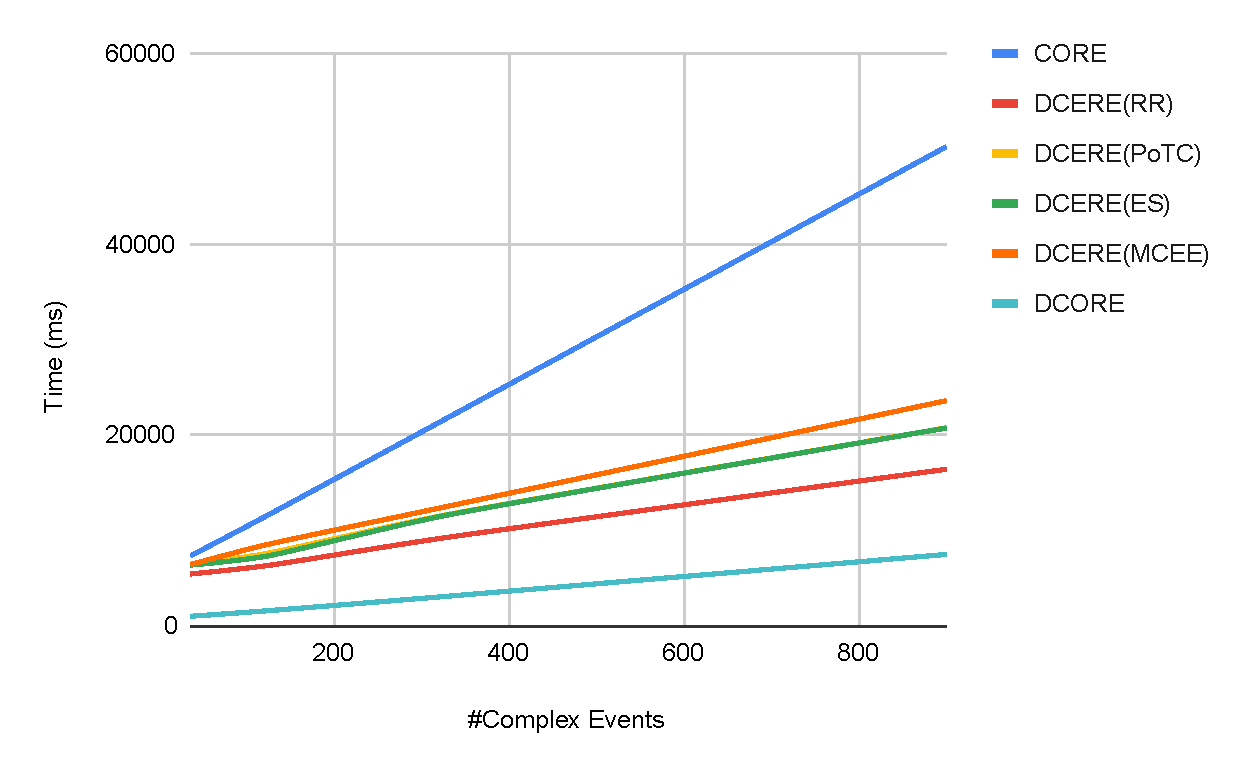
\includegraphics[width=\textwidth]{experiment_1_chart_1}
            \tiny (a) $Q_{1}$
        \end{subfigure}
        \begin{subfigure}[b]{0.40\textwidth}
            \centering
            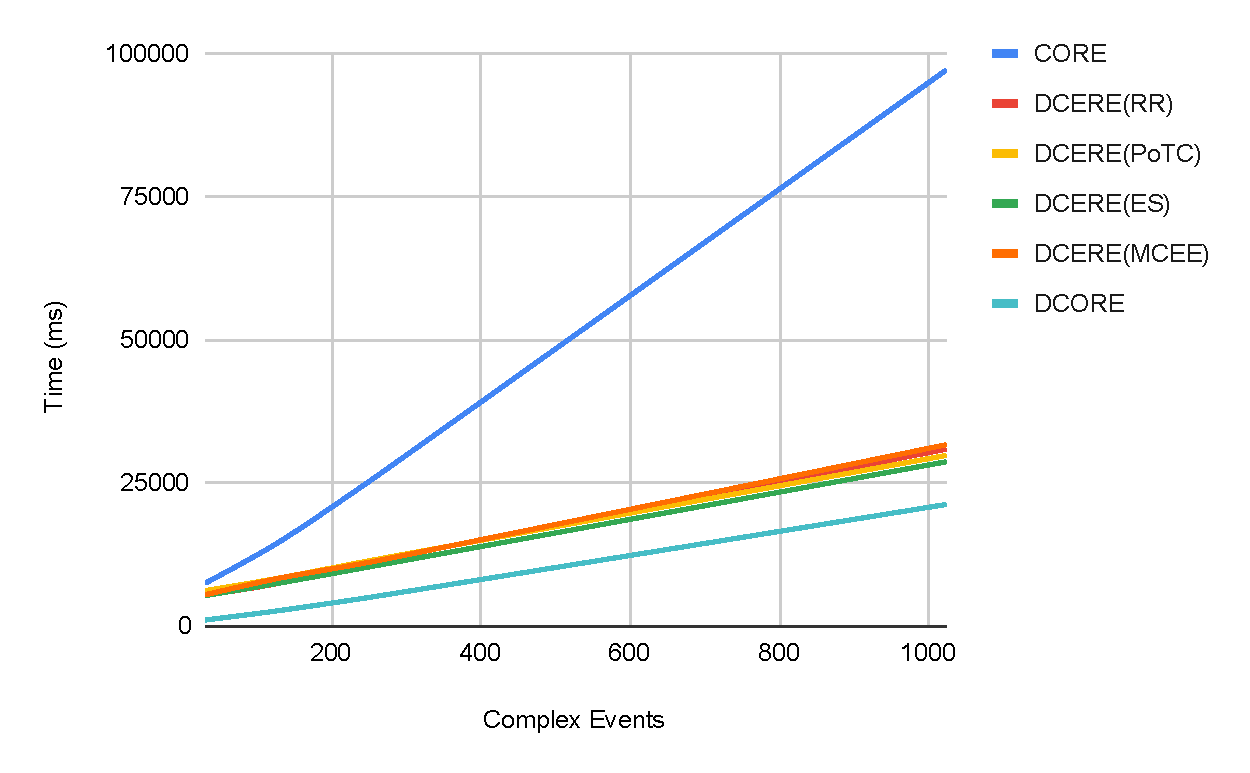
\includegraphics[width=\textwidth]{experiment_1_chart_2}
            \tiny (b) $Q_{2}$
        \end{subfigure}
        \begin{center}
          \begin{subfigure}[b]{0.40\textwidth}
              \centering
              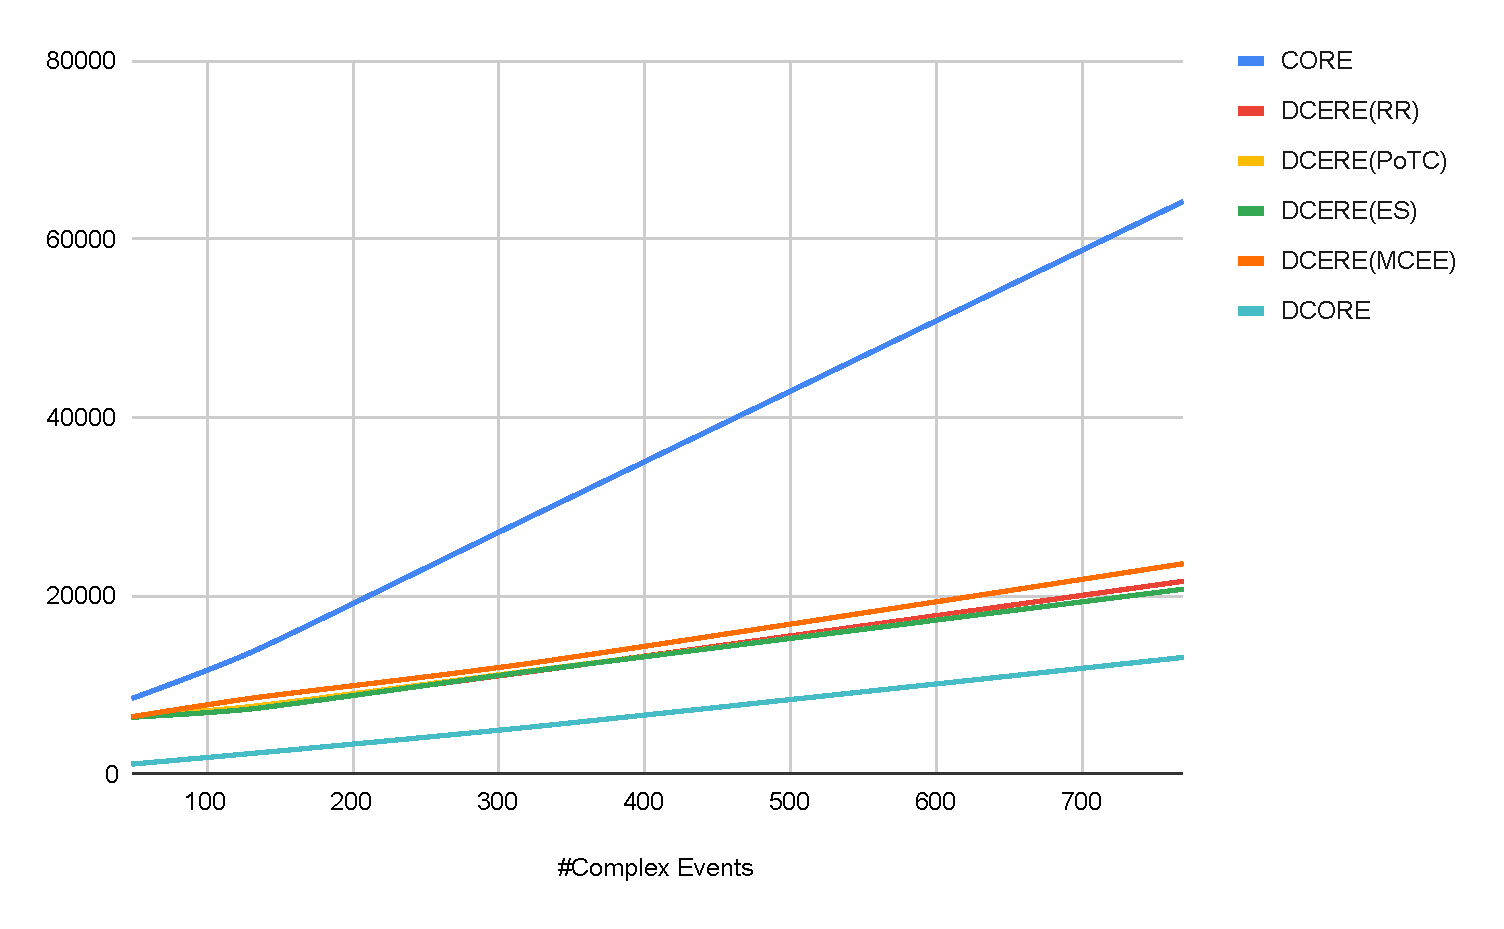
\includegraphics[width=\textwidth]{experiment_1_chart_3}
              \tiny (c) $Q_{3}$
          \end{subfigure}
        \end{center}
    \end{figure}
  \end{block}
\end{frame}

%%%%%%%%%%%%%%%%%%%%%%

\begin{frame}{Experiments}
  \begin{block}{On the scalability of the framework}
    \begin{figure}[H]
        \centering
        \begin{subfigure}[b]{0.49\textwidth}
            \centering
            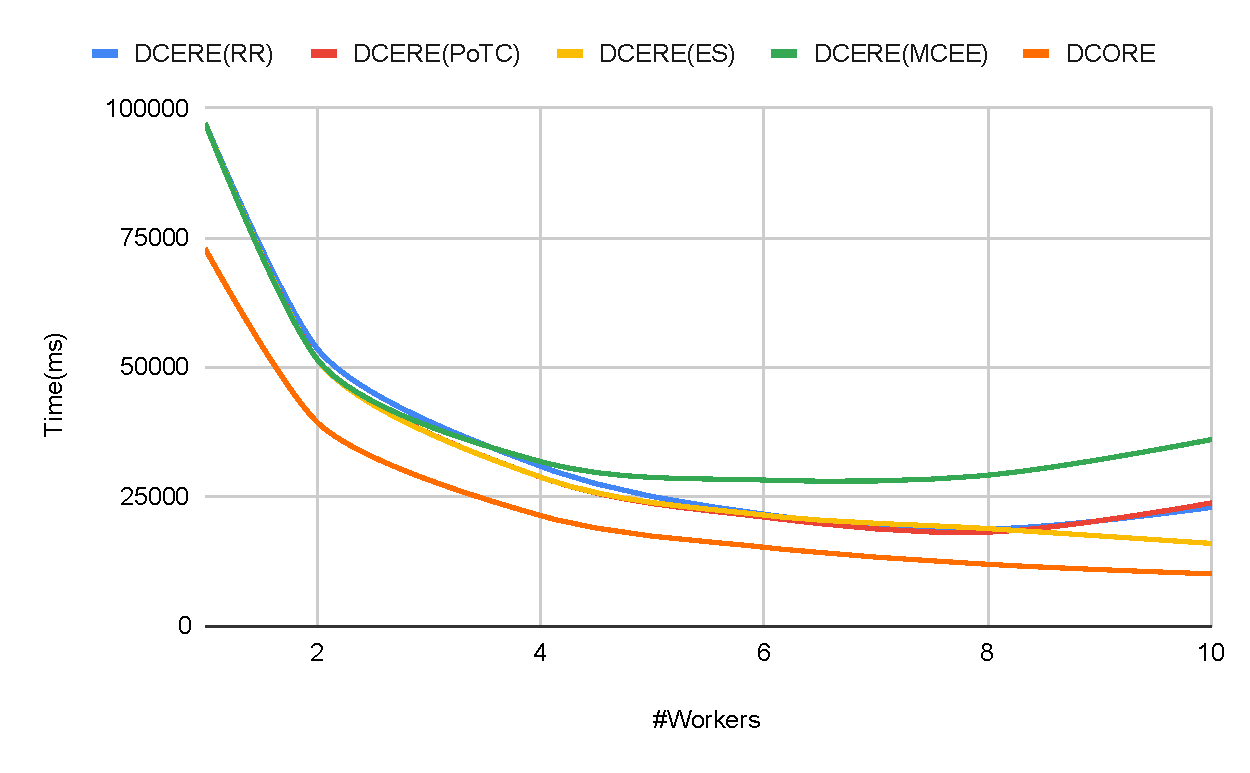
\includegraphics[width=\textwidth]{experiment_3_chart_1}
            \tiny (a) $1024$ complex events
        \end{subfigure}
        \begin{subfigure}[b]{0.49\textwidth}
            \centering
            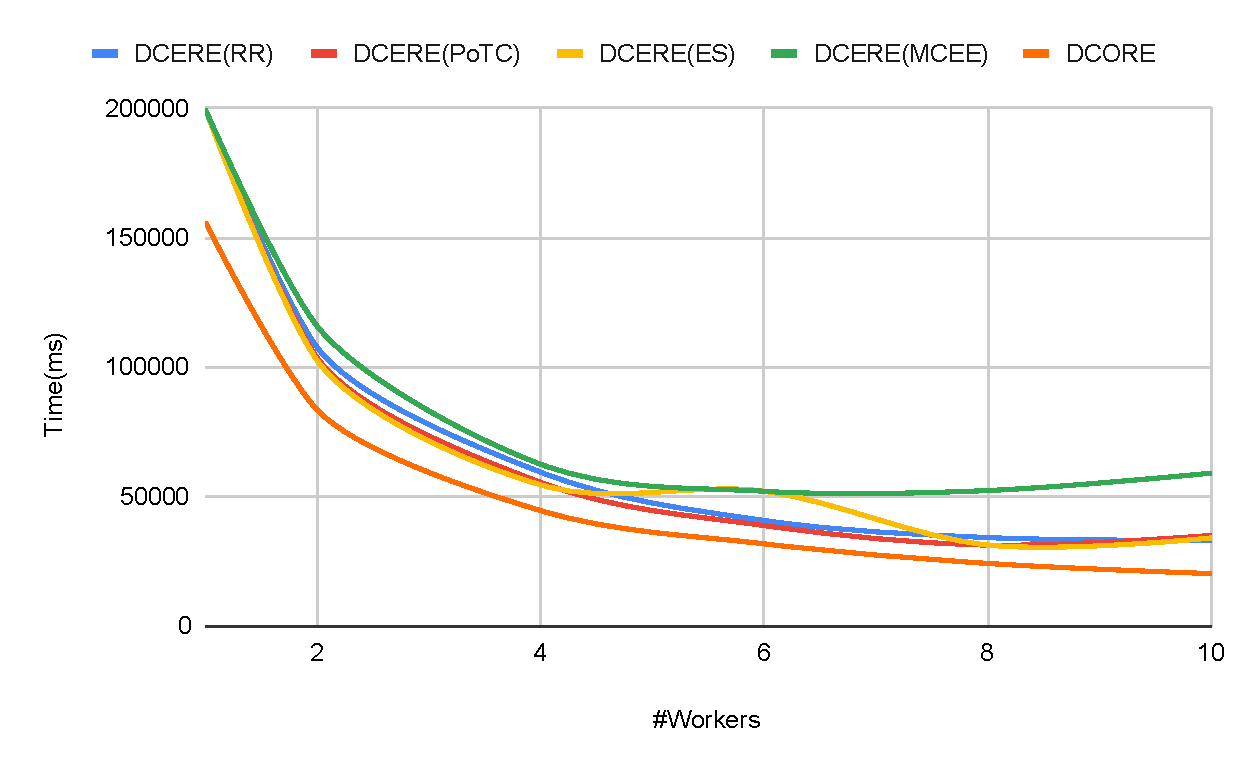
\includegraphics[width=\textwidth]{experiment_3_chart_2}
            \tiny (b) $2048$ complex events
        \end{subfigure}
    \end{figure}
  \end{block}
\end{frame}

%%%%%%%%%%%%%%%%%%%%%%

\begin{frame}{Experiments}
  \begin{block}{On DCORE under heavy loads}
    \begin{figure}[H]
        \centering
        \begin{subfigure}[b]{0.4\textwidth}
            \centering
            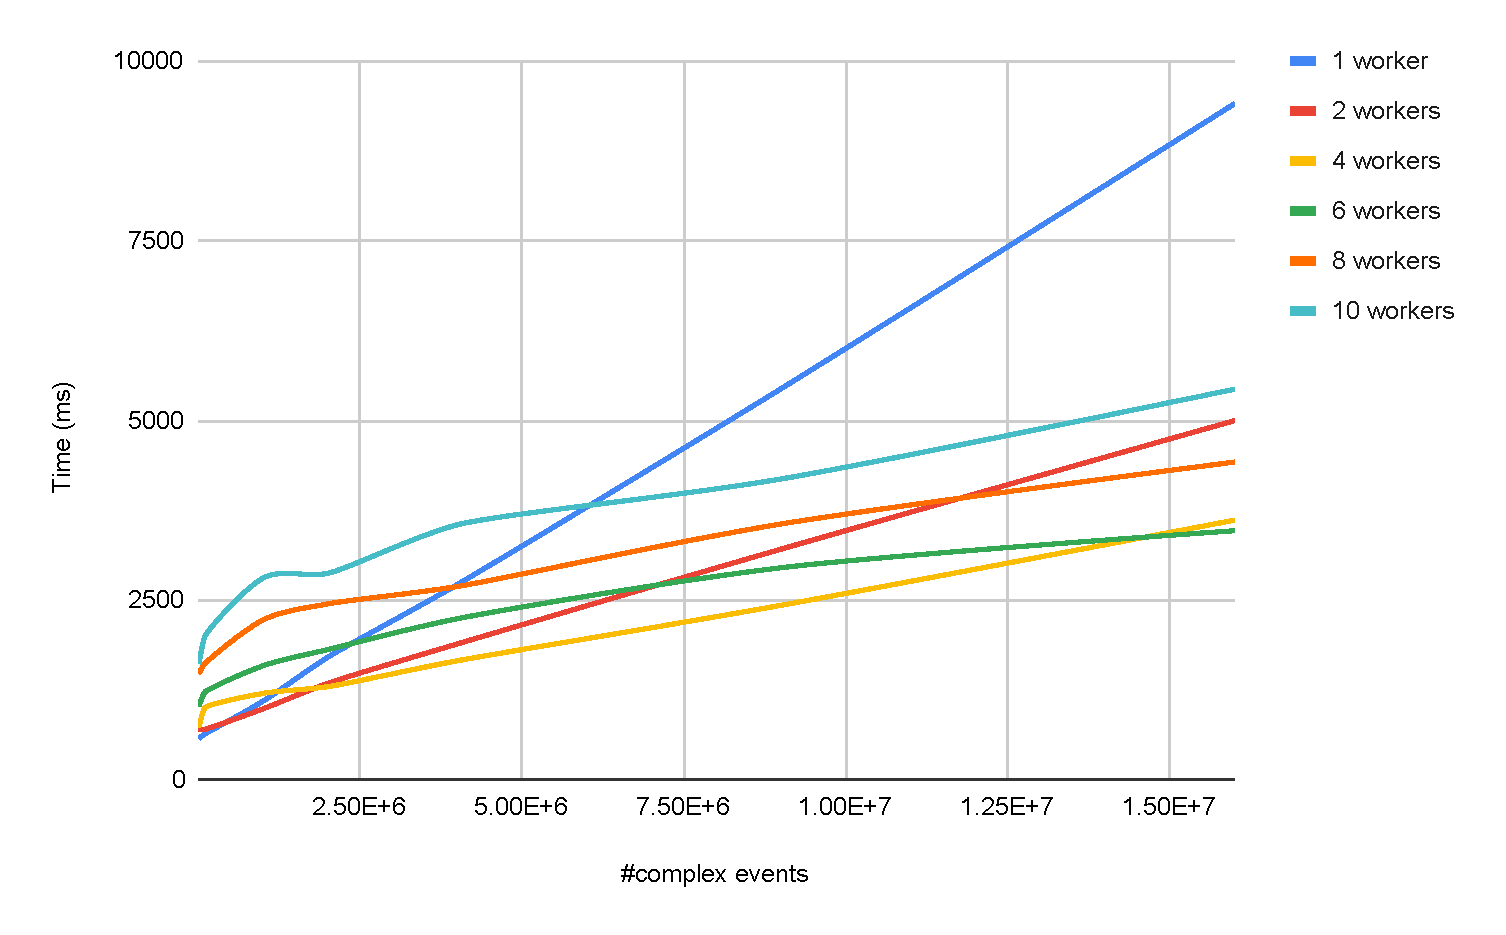
\includegraphics[width=\textwidth]{experiment_4_chart_1}
            \tiny (a) $Q_{1}$
        \end{subfigure}
        \begin{subfigure}[b]{0.4\textwidth}
            \centering
            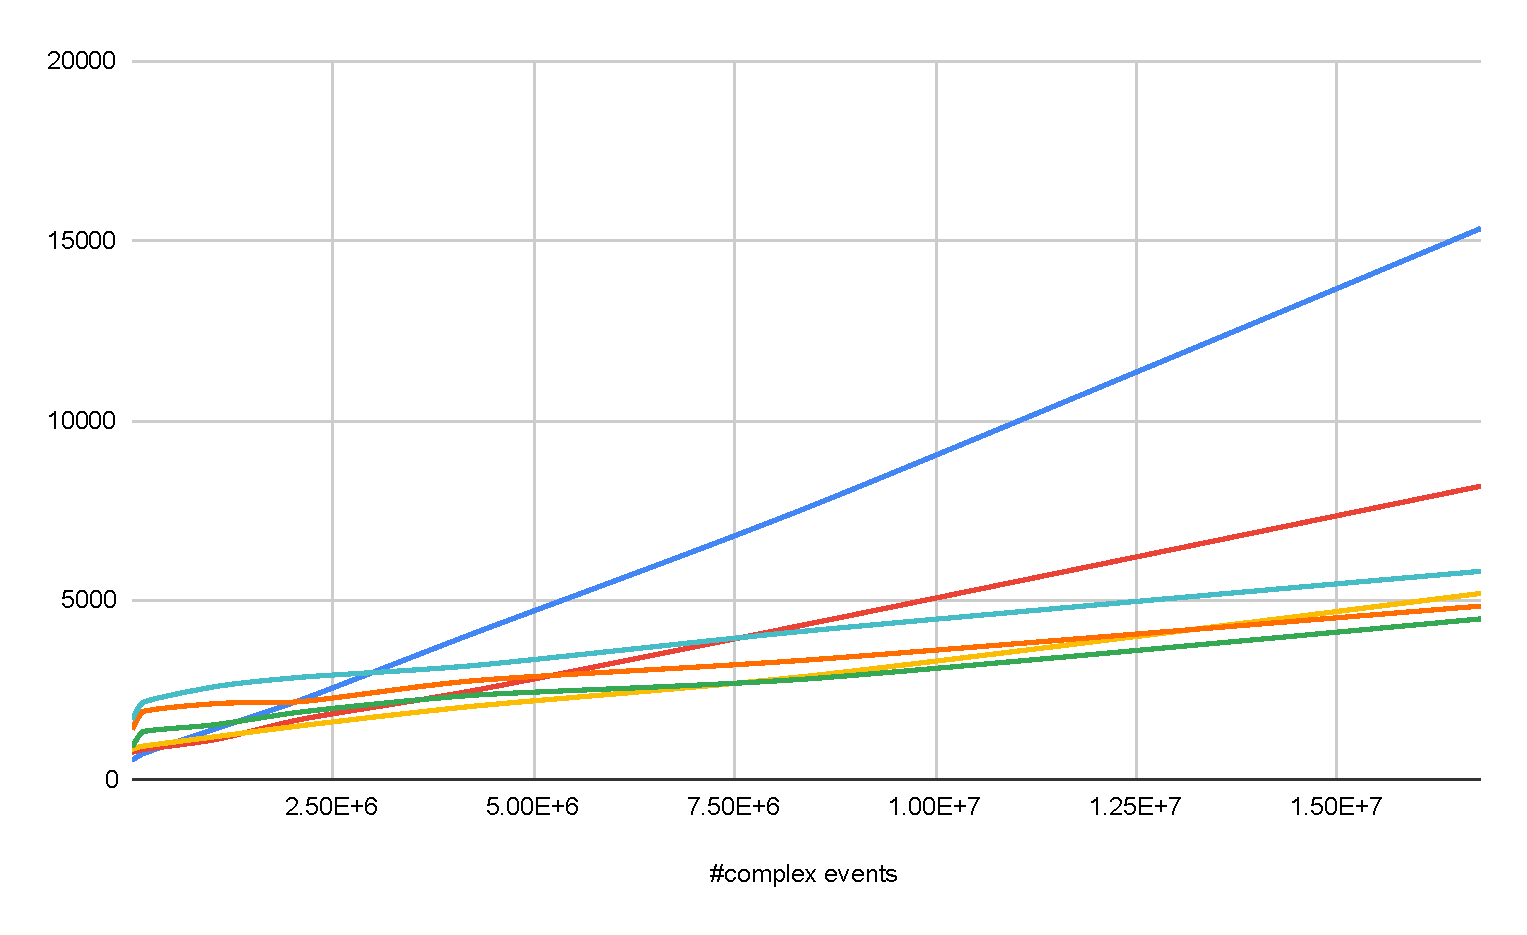
\includegraphics[width=\textwidth]{experiment_4_chart_2}
            \tiny (b) $Q_{2}$
        \end{subfigure}
        \begin{center}
        \begin{subfigure}[b]{0.4\textwidth}
            \centering
            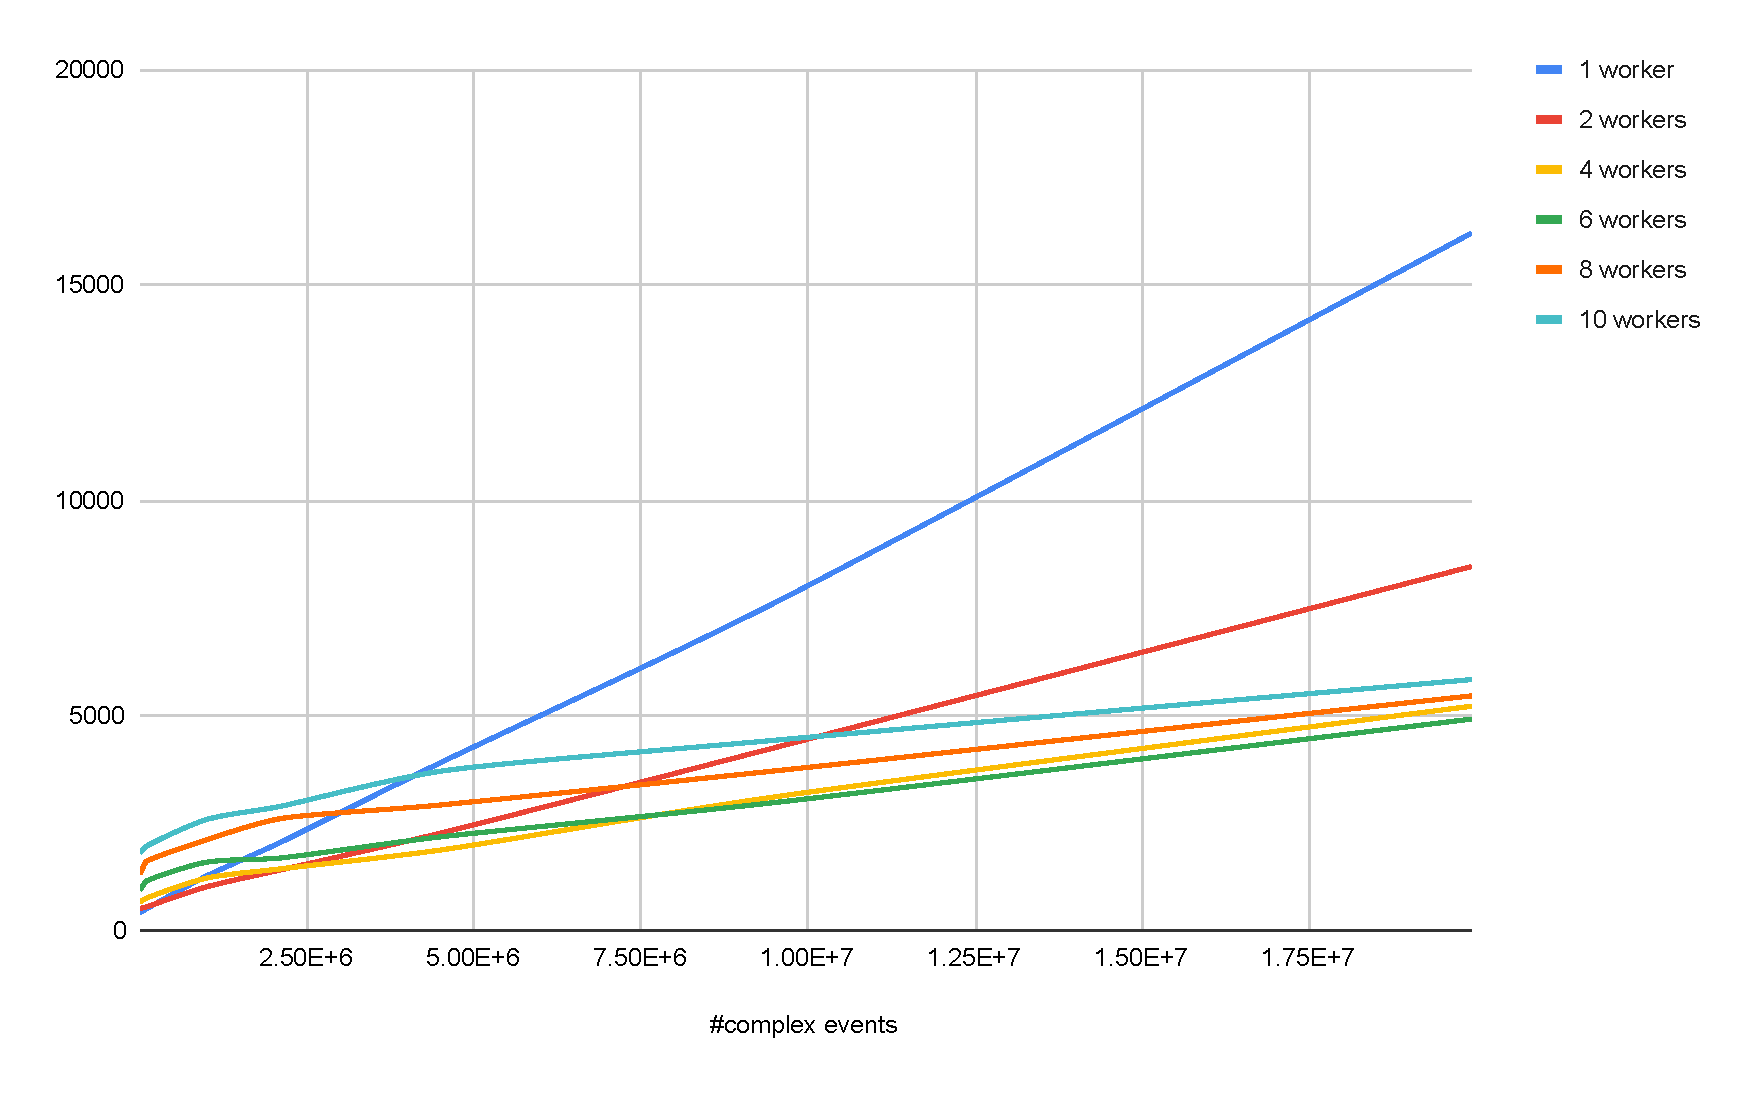
\includegraphics[width=\textwidth]{experiment_4_chart_3}
            \tiny (c) $Q_{3}$
        \end{subfigure}
        \end{center}
    \end{figure}
  \end{block}
\end{frame}


%%%%%%%%%%%%%%%%%%%%%%%%%%%%%%%%%%%%%%%%%%%%%%%%%%%%%%%%%%%%%%%%%%
%%%%%%%%%%%%%%%%%%%%%%%%%%%%%%%%%%%%%%%%%%%%%%%%%%%%%%%%%%%%%%%%%%

\section{Conclusions and Future Work}

\begin{frame}{Conclusions \& future work}
  \begin{block}{Conclusions}
   \begin{itemize}
     \item We presented:
        \begin{itemize}
          \item A framework for distributed CER.
          \pause
          \item Two implementations: DCERE and DCORE.
          \pause
          \item A distributed evaluation algorithm for DCORE.
        \end{itemize}
     \pause
     \item We showed that both implementations of our framework outperform its competitors on queries with complex predicates.
   \end{itemize}
  \end{block}
\end{frame}

%%%%%%%%%%%%%%%%%%%%%%

\begin{frame}{Conclusions \& future work}
  \begin{block}{Future Work}
   \begin{itemize}
     \item Extend our framework with a generic rewrite and refine algorithms.
     \pause
     \item Extend our distributed evaluation algorithm to take into account time windows.
     \pause
     \item Explorer the capabilities offered by other automatas (e.g., register and data automata).
   \end{itemize}
  \end{block}
\end{frame}

%%%%%%%%%%%%%%%%%%%%%%

\begin{frame}[c]{ }
  \centering
  \huge Questions ?
\end{frame}

%%%%%%%%%%%%%%%%%%%%%%%%%%%%%%%%%%%%%%%%%%%%%%%%%%%%%%%%%%%%%%%%%%
%%%%%%%%%%%%%%%%%%%%%%%%%%%%%%%%%%%%%%%%%%%%%%%%%%%%%%%%%%%%%%%%%%

\begin{frame}[allowframebreaks]
  \frametitle{Bibliography}
  \bibliographystyle{unsrt}
  \bibliography{bibliography}
\end{frame}

\end{document}

